%!TEX root = ../thesis.tex
\markboth{Appendix}{APPENDIX}
\begin{appendices}

\chapter{User Generated Results using DemoDraw}
\renewcommand\thefigure{A.\arabic{figure}}
\setcounter{figure}{0}
\begin{figure}
   \begin{minipage}[b]{1.0\textwidth}
     \centering
    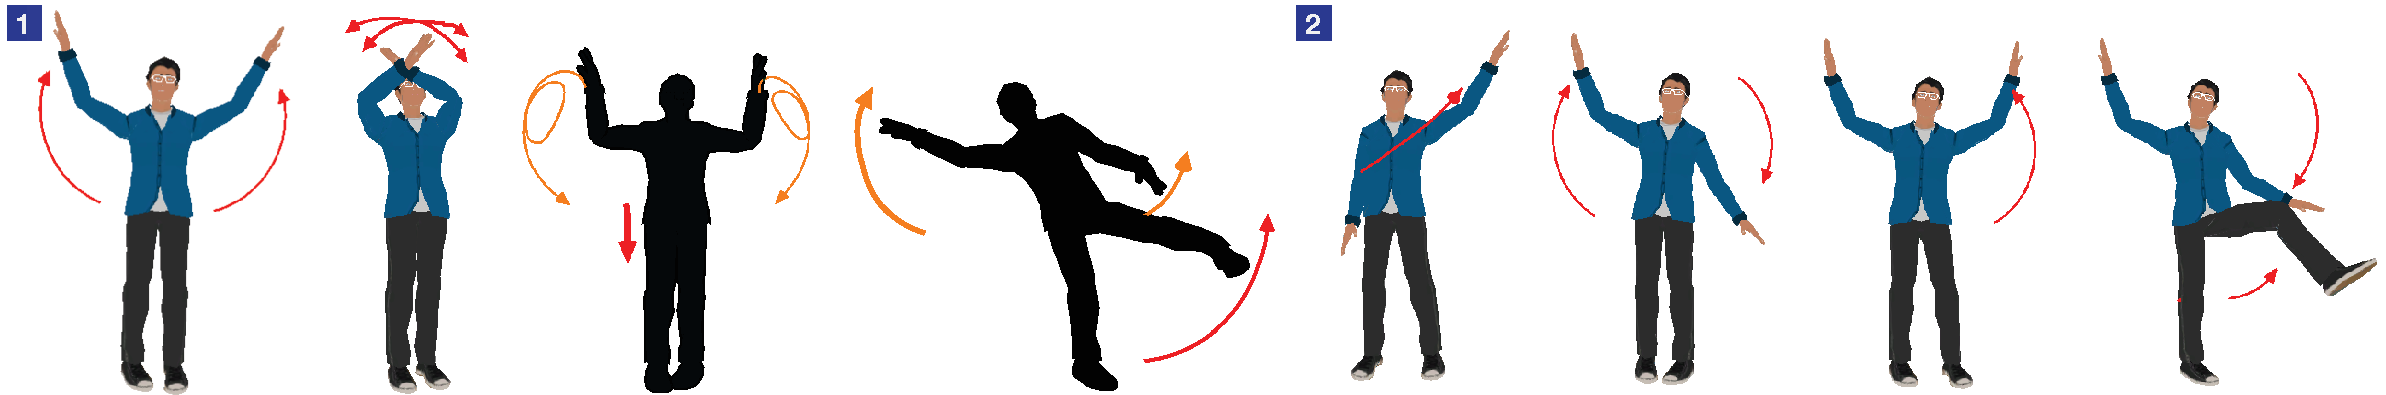
\includegraphics[width=\columnwidth]{\demodraw/fig/study1/study1_tasks}
    \caption{Tasks provided in Study 1: We showed the printouts of these two sets of 4-step motions generated by DemoDraw using both the \phaseI{} and the \phaseII{}. We asked participants to re-perform in front of a camera.}
    \label{fig:study_review_tasks}
   \end{minipage}

   \vspace{6mm}
   \begin{minipage}[b]{1.0\textwidth}
     \centering
    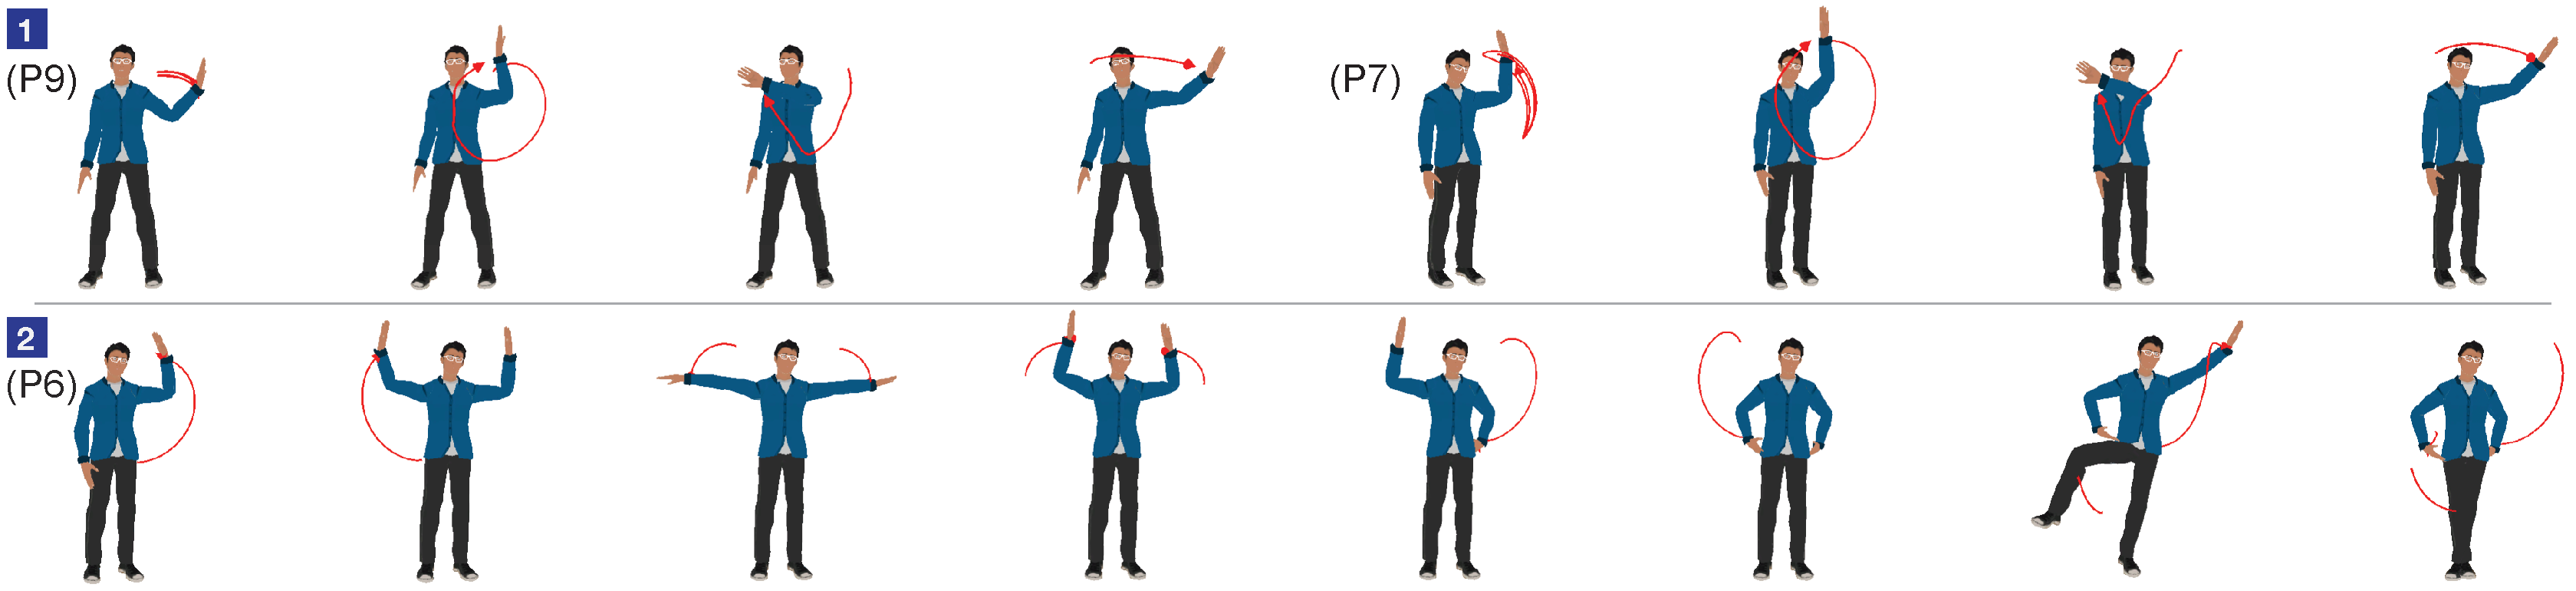
\includegraphics[width=\columnwidth]{\demodraw/fig/study2/study2_tasks}
    \caption{Step-by-step illustrations generated by participants in Study 2 using the \phaseI{}: 1) Results from P9 and P6 showing the same four gestures of a gestural interface in task 1, and 2) Results from P6 showing 8-step moves in task 2.}
    \label{fig:study_authoring_tasks}
   \end{minipage}

   \vspace{6mm}
   \begin{minipage}[b]{1.0\textwidth}
     \centering
    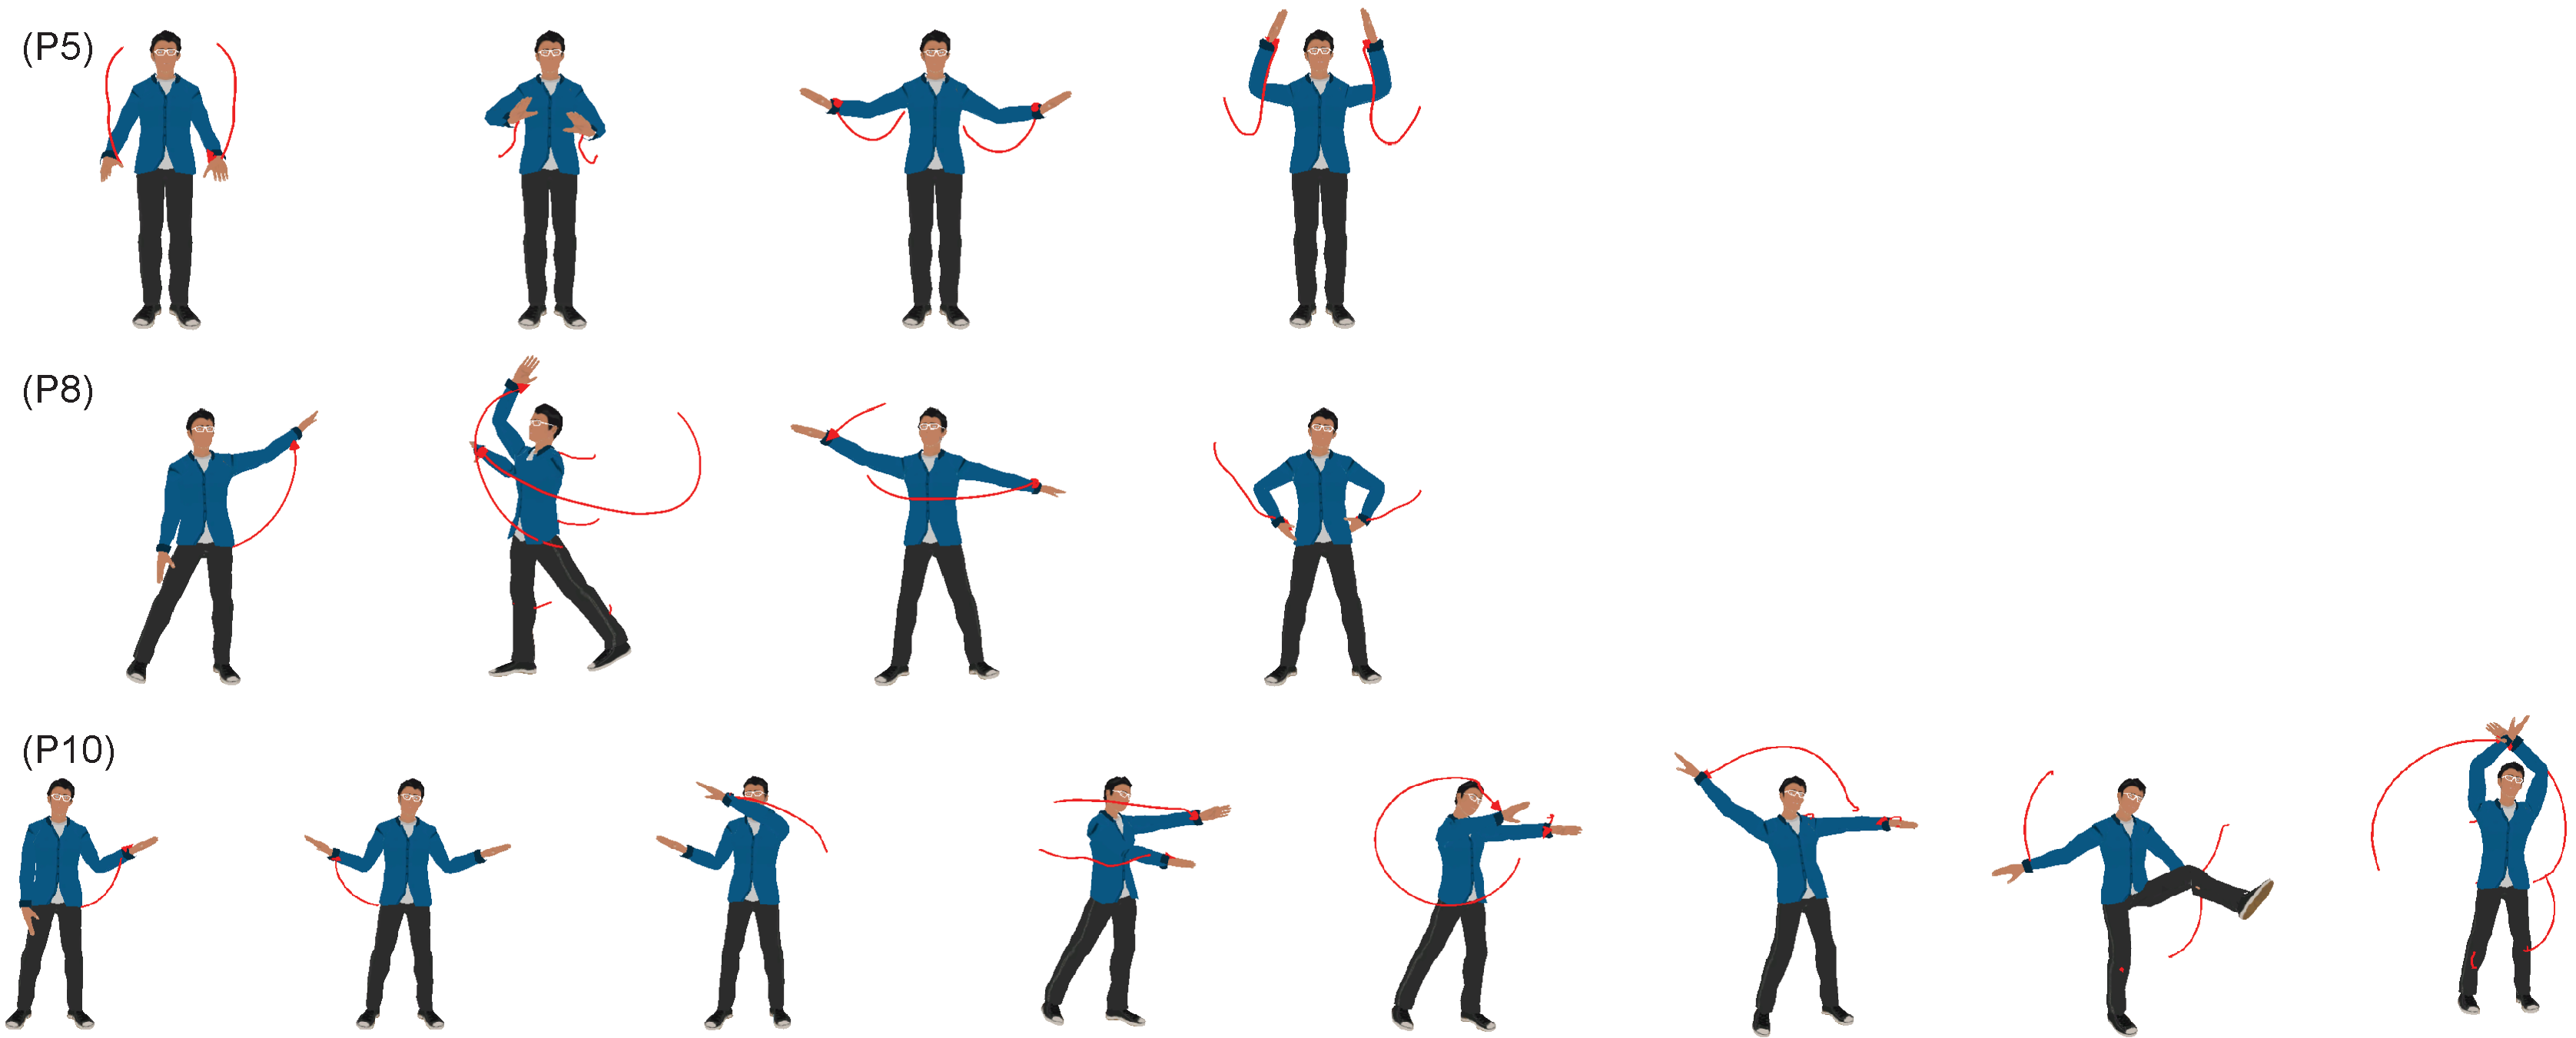
\includegraphics[width=\columnwidth]{\demodraw/fig/study2/study2_open}
    \caption{Selected illustrations from the open-ended task created by three different participants using the using \phaseI{} in Study 2: P5 performed to conduct a 4/4 beat pattern; P8 and P10 each performed four and eight free moves.}
    \label{fig:open_ended_examples}
   \end{minipage}
 \end{figure}

\end{appendices}
